\documentclass[10pt]{extarticle}
\usepackage{graphicx}
\usepackage[margin=.5in]{geometry}
\usepackage{multicol}
\usepackage{helvet}
\usepackage{algorithm}
\usepackage[noend]{algpseudocode}
\usepackage{subcaption}

\begin{document}
	
	\twocolumn
	
	\title{Controller Assignment}
	\author{Shadman Protik\\Talha Ibn Aziz }
	\date{10/4/2018}
	\maketitle
	
	\section{Problem Statement} \label{prob}
	Let a network be represented by a graph $G=(S,L)$, where $S$ is the set of switches or nodes and $L$ is the list of connecting edges. This network is to be divided into $k$ disjoint sets of switches $S_{i:i=1,2,3...}$ and a controller is to be assigned to each set $S_i$ such that the following four conditions are met:
	\begin{enumerate}
		\item The latency from each controller to the nodes of $S_i$ is minimized.
		\item The latency from each controller to other controllers is minimized.
		\item The reliability of the network is maximized.
		\item The number of controllers, $k$ needs to be minimized as much as possible (cost efficiency). 
	\end{enumerate}
	
	This is called the Controller Placement Problem.
	Therefore, there are more than one parameters which need to be optimized. Most of the works\cite{dbcp} defined this problem as a multi-objective combinatorial optimization problem.
	
	Controller Assignment can be divided into two phases:
	\begin{itemize}
		\item Clustering
		\item Controller Selection
	\end{itemize}
	
	Clustering is the process of determining the number of controllers $k$ and $k$ sets of disjoint switches or 'clusters' such that the target objectives 1 and 4 mentioned in section \ref{prob} are reached. We worked with two well known algorithms DBCP\cite{dbcp} and SPICi\cite{spici} that cluster a network very efficiently to reach different goals. And we proposed a new algorithm Inverse-SPICi which is a variation of SPICi. These three algorithms have been explained in details in sections \ref{algo:dbcp}, \ref{algo:spici} and \ref{algo:ispici} respectively.
	
	Controller selection is the method to select a controller from each cluster that has been formed due to the clustering algorithms. DBCP has used a method of controller selection which has been described in section \ref{dbcp:consel}.
	
	\section{Algorithm 1: DBCP\cite{dbcp}} \label{algo:dbcp}
	
	\subsection{Clustering} \label{dbcp:cluster}
	DBCP (Density Based Controller Placement) clusters a network using the local density of a node and the minimum distance to a higher density node.
	\begin{equation} \label{dbcp:density}
	\rho_i=\sum_j\chi(d_{ij}-d_c)
	\end{equation}
	The local density (equation \ref{dbcp:density}) of a node $s$ is the count of all the nodes which are at most $d_c$ distance away from $s$ and is denoted by $\rho_s$. The threshold $d_c$ is a distance used to set a limit to the cluster diameter and consequently to find an approximate to the optimal value of $k$.
	Here $d_{ij}$ gives the minimum distance between nodes $i$ and $j$. The value of $\chi(x)$ is 1 only for $d_{ij}<d_c$ that is when $x<0$ and is 0 otherwise. Thus $\rho_i$ is the number of nodes that can be reached from node $i$ by traversing at most distance $d_c$.
	
	The minimum distance to a higher density node is represented by the term $\delta_s$ for a node $s$. For the node with highest density there is no other node with higher density and so only for that node, $\delta_s$ holds the distance of the farthest node from $s$.
	
	For a set of nodes $S$ with a set of edges $L$ among them in a graph $G=(S,L)$ they fixed a value of $k$, that is the number of clusters to be formed each with one controller. They formed the clusters and selected a node as controller based on the values of $\rho_s$ and $\delta_s$. The more the values $\rho_s$ and $\delta_s$ for a node $s$, the more it's chances are for being selected as the controller. The method for selecting the cluster head or controller of each sub-network is explained further in detail in the section \ref{dbcp:consel}.
	
	\begin{algorithm}
		\caption{: Density Based Controller Placement}\label{euclid}
		\begin{algorithmic}[1]
			\Procedure{DBCP}{S,L} \\
			$k \gets 0$ \\
			\textbf{for $s$ in S:}
			\State $\rho_s=\sum_{j\in S}\chi(d_{sj}-d_c)$ \\
			\textbf{end for} \\
			\textbf{for $s$ in S:}
			\State $\delta_s=\min_{i:i\in S,p_i>p_s}(d_{is})$ \\
			\textbf{end for} \\
			$\delta \gets \frac{1}{|S|}\sum_{s\in S}\delta_s$ \\
			\textbf{for s in S:}
			\If {$\delta_s>\delta$}	
			\State $k = k + 1$
			\State $s \gets newcluster$
			\Else
			\State $s \gets cluster of nearest higher density$
			\EndIf \\
			\textbf{end for}
			\EndProcedure
		\end{algorithmic}
	\end{algorithm}
	
	In the \cite{dbcp} they used hop count as the metric for latency. That is all distances were calculated considering node to node distance a constant value of 1 (1 hop). We also considered the case if it is not constant. Therefore we implemented the same algorithm for the case where node to node distance can be any positive real number and used that as the distance metric. This numeric value can represent the bandwidth of that link or channel. It can also represent the transmission rate of the link. We named this new implementation Weighted Density Based Controller Placement or W-DBCP and included it in the results analysis and algorithm comparison of section \ref{comp}.
	
	This algorithm has a few drawbacks which are also pointed out with example graphs in the section \ref{comp}.
	
	\subsection{Controller Selection} \label{dbcp:consel}
	DBCP uses three metrics to determine the controller for a cluster. The cluster head of a network is a node from where the cluster formation starts. A controller is the node which will act as the control plane for that specific sub-network data plane (rest of the switches). We selected the controllers for the sub-networks using the same metrics as DBCP. These three metrics are described in the following sections.
	
	\subsubsection{Controller-to-switch latency}
	For a sub-network graph $S(\theta)$, the average propagation latency for a placement location $v:v\in S(\theta)$ of a controller θ is calculated as:
	\begin{equation}	\label{pi1}
	\pi_{avglatency}(S(\theta)) = \min_{v\in S(\theta)} \frac{1}{|S(\theta)|} \sum_{s\in S(\theta)}d(v,s)
	\end{equation}
	
	Thus the average of the distances of the node $v$ from all other nodes is calculated. To select a node as the controller, $\pi_{avglatency}$ must be minimum.
	For the worst case scenario another metric is defined. This metric is denoted by $\pi_{maxlatency}$.
	\begin{equation}	\label{pi2}
	\pi_{maxlatency}(S(\theta)) = \min_{v\in S(\theta)} \max_{s\in S(\theta)}d(v,s)
	\end{equation}
	
	This is the maximum of the distances of the node $v$ from all the other nodes $s:s\in S(\theta)$ in the cluster $S(\theta)$. This maximum must be minimized for a cluster. Therefore all nodes are considered when calculating $\pi_{maxlatency}$ and only the switch with the minimum value is selected as controller.
	
	\subsubsection{Inter-controller latency}
	The inter controller latency must be reduced as much as possible when selecting controller. But the controller to controller distance cannot be determined when the controllers are yet to be selected. Thus a new metric is used which is denoted by $\pi_{inter\_controller}$.
	\begin{equation}	\label{pi3}
	\pi_{inter\_controller}(S(\theta)) = \min_{v\in S(\theta)} \frac{1}{|S|} \sum_{s\in (S-S(\theta))}d(v,s)
	\end{equation}
	
	Thus it is the sum of the distances of the node $v$ of the cluster $S(\theta)$ to all the nodes of other clusters divided by the total number of nodes in the network. The node which has the minimum value of $\pi_{inter\_controller}$ is selected as the controller $\theta$.
	
	\subsubsection{Total Latency}
	This is the final metric which is the sum of all three previous metrics in equations (\ref{pi1}), (\ref{pi2}) and (\ref{pi3}).
	\begin{equation}
	\pi_{latency} = \pi_{avglatency} + \pi_{maxlatency} + \pi_{inter\_controller}
	\end{equation}	\label{pi4}
	\[\pi_{latency}S(\theta)=\min_{v\in S(\theta)}(\frac{1}{|S(\theta)|} \sum_{s\in S(\theta)}d(v,s) + \max_{s\in S(\theta)}d(v,s)\]
	
	\begin{equation}
	+ \frac{1}{|S|} \sum_{s\in (S-S(\theta))}d(v,s))
	\end{equation}
	Thus for each node in a cluster $S(\theta)$ we find the value of $\pi_{latency}(S(\theta))$ and then we select the node with minimum $\pi_{latency}$ as the controller $\theta$ of the cluster.
	
	\subsection{Drawbacks}
	There are quite a few drawbacks of this network clustering algorithm. These are described in brief as follows:
	
	\begin{enumerate}
		\item For a densely connected graph almost every other node can be reached from a particular node in 1 or 2 hops. As such the only possible values of constant $d_c$ are 1 or 2. For the value of constant $d_c=2$ all the nodes have the same density and therefore average minimum distance to higher density nodes is equal to minimum distance to higher density node for all the nodes and so according to the algorithm $k=0$ which basically means there are no clusters, which is not possible.
		\item For $d_c$ equal to 1 we are just basically calculating density based on incident degree of a node. Thus only 2 minimum distances to higher density nodes are possible which are 1 and 2.
		There are only two possible results in this case, one is $k=0$ as mentioned in previous point and the other is a certain number of controllers. Therefore there is very less variation in the number of clusters.
		\item The Algorithm selects the cluster for a node following the condition of line 15 of algorithm \ref{algo:dbcp}. That is an unclustered node is assigned a cluster based on the cluster of it's nearest higher density. This creates a problem if a loop occurs such that there are two switches $s_1$ and $s_2$, and $s_1$ has nearest higher density $s_2$ and $s_2$ has nearest higher density $s_1$. This is possible when one switch is of highest density and other is farthest from the switch with highest density which is quite often in the case of dense graphs.
	\end{enumerate}
	
	We showed the drawbacks using different scenarios again in section \ref{comp}.
	
	\section{Algorithm 2: SPICi}	\label{algo:spici}
	
	SPICi ('spicy', Speed and Performance In Clustering) clusters a connected undirected graph $G=(V,E)$ with edges that have confidence values of the continuous range $(0,1)$ so that each cluster has a seed as center from which clustering starts. These edges can be represented by $w_{u,v}$ such that $u,v\in V$, $w_{u,v}\in E$ and $0\le w_{u,v}\le1$. It works with three variables and two thresholds. The three variables can be defined as the weighted degree of a node $d_w$, the density of a set of nodes $S$ and the support of a node $u\in V$ with respect to a set of nodes $S$:
	\begin{equation}
	d_w(u)_{u\in V} = \sum_{v:v\in V,(u,v) \in E}w_{u,v}
	\end{equation}
	
	Therefore $d_w(u)_{u\in V}$ is the sum of all the weights of the edges that connect $u$ with any other adjacent node $v$ of the graph $G=(V,E)$.
	
	\begin{equation}
	density(S) = \frac{\sum_{(u,v)\in E}w_{u,v}}{|S|*(|S|-1)/2} 
	\end{equation}
	
	In other words, $density(S)$ is the sum of the edges that connect every node $u$ with every other node $v$ of $S$ divided by the number of total possible nodes that is $|S|*(|S|-1)/2$ where $|S|$ is the number of nodes present in the set of nodes $S$.
	
	\begin{equation} \label{support}
	support(u,S) = \sum_{v\in S} w_{u,v}
	\end{equation}
	And $support(u,S)$ is the sum of the edges that connect a node $u$ with the nodes adjacent to it present in the set of nodes $S$.
	
	The thresholds are: $T_s$ which determines whether a node is to be included in the cluster based on the cluster size and the connectivity of the node to the cluster and: $T_d$ which includes a node to the cluster based on the density increased when the node is added.
	\begin{algorithm}
		\caption{: SPICi}\label{spicicode}
		\begin{algorithmic}[1]
			\Procedure{Search}{V,E} \\
			\textbf{Initialize} $DegreeQ = V$ \\
			\textbf{While} $DegreeQ \neq empty$
			\State Extract u from DegreeQ with largest $d_w(u)$
			\If {there is $v_{v:v,u\in E}\in DegreeQ$}
			\State $v \gets secondseed(DegreeQ,E,u)$
			\If {$v\neq null$} $S \gets Expand(u,v)$
			\EndIf
			\Else 
			\State $S \gets \{u\}$
			\EndIf
			\State $V \gets V - S $
			\State $Degree Q \gets Degree Q - S$
			\State $d_w(t)_{t:t\in DegreeQ,(t,s)_{s\in S}\in E} = d_w(t) - support(t,S)$
			\EndProcedure\\
			\Procedure{SecondSeed}{V,E,u} \\
			$bin[i]_{i:i=(1,5)} \gets s_{s:s\in V,(s,u)\in E}$ \\
			\textbf{for i = 1 to 5}
			\If {$bin[i] \neq empty$}
			\State \Return $v$ \textbf{if} $d_w(v)=\max_{s:s\in bin[i]}{d_w(s)}$
			\EndIf\\
			\Return $null$
			\EndProcedure\\
			\Procedure{Expand}{V,E,u,v}\\
			\textbf{Initialize} the cluster $S \gets \{u,v\}$ \\
			\textbf{Initialize} $CandidateQ = S_{S:s\in S,(s,u),(s,v)\in E}$\\
			\textbf{While} $CandidateQ \neq empty$
			\State Extract $t$ from Candidate with highest $support(t,S)$
			\If {$support(t,S)\geq T_s*|S|*density(S)$ and
				$density(S + t)> T_d$}
			\State $S\gets S+\{t\}$
			\State $CanditateQ \gets CandidateQ + \{s_{s:(s,t)\in E}\}$
			\State $CandidateQ \gets CandidateQ - \{s_{s:s\not\in CandidateQ}\}$
			\Else
			\State break from loop
			\EndIf \\
			\Return S
			\EndProcedure
		\end{algorithmic}
	\end{algorithm}
	The nodes are added to bins 1,2,3,4 and 5 respectively if their connected edge value $w_{s,u}\leq0.2,0.3,0.4$ and $0.5$ such that $s,u\in V$ and $(s,u)\in E$.
	
	
	\section{Proposed 1: I-SPICi} \label{algo:ispici}
	
	The algorithm I-SPICi or Inverse-SPICi is a derivative of SPICi and one of our proposed algorithms. It has two steps \emph{Clustering} and \emph{Controller Selection} which are given as follows.
	
	\subsection{Clustering}
	This algorithm is taken from SPICi without any post processing or modification except that the cost is taken in an inverse manner. If the graph is represented by $G=(V,E)$ where $V$ is the set of nodes and $E$ is the set of edges containing edge costs $w_{u,v}$ such that $u,v\in V$ and $(u,v)\in E$ the costs can be expressed by the following equations.
	\begin{equation}
	max\_cost = \max_{u,v\in E}(w_{u,v}+1)
	\end{equation}
	\begin{equation}
	cost_{u,v} = max\_cost - w_{u,v}
	\end{equation}
	
	Here $max\_cost$ is the maximum edge distance or cost of all the edges present in the graph. To each edge cost, 1 is added before calculating the maximum cost so that the selected maximum cost ($max\_cost$) is greater than the actual maximum cost. Therefore after subtracting each of the edge costs from this maximum cost will not result in zero even for the actual maximum cost. When all the costs have been reassigned, this results in the costs being reversed for any pair of adjacent nodes $u,v:(u,v)\in E$. 
	
	Thus the highest edge cost becomes the lowest and the lowest edge cost becomes the highest.
	This cost acts as the new edge value when calculating the values of weighted degree, support and density of the required set of nodes.
	
	\subsection{Controller Selection}
	We selected the controller for a cluster by calculating the $support(u,S)$ (as expressed in equation (\ref{support})) for a set of nodes $S$ which in this case is the cluster in consideration and a node $u:u\in S$. Each node gives a value of support and we selected the node with the maximum support. This can be improved further if we again take the original edge costs instead of the reversed ones or if we use the same controller selection method as used in DBCP.
	
	\section{Proposed 2: G-SPICi} \label{algo:gspici}
	
	\subsection{Clustering}
	This algorithm is  also taken from SPICi without any post processing. The only modification is that all the nodes of a cluster except the \textbf{first seed protein} (as per stated in \cite{spici}) or \textbf{cluster head} (in terms of clustering terminology), are selected using the same method. The node with maximum support with respect to the current cluster that is being built is selected each time. Therefore there would be no second seed selection function. The pseudo-code would also be changed. The changed pseudo-code is given below in algorithm \ref{gspicicode}.
	\begin{algorithm}
		\caption{:Greedy-SPICi}\label{gspicicode}
		\begin{algorithmic}[1]
			\Procedure{Search}{V,E} \\
			\textbf{Initialize} $DegreeQ = V$ \\
			\textbf{While} $DegreeQ \neq empty$
			\State Extract u from DegreeQ with largest $d_w(u)$
			\State $S \gets Expand(u)$
			\State $V \gets V - S $
			\State $Degree Q \gets Degree Q - S$
			\State $d_w(t)_{t:t\in DegreeQ,(t,s)_{s\in S}\in E} = d_w(t) - support(t,S)$
			\EndProcedure\\
			\Procedure{Expand}{V,E,u}\\
			\textbf{Initialize} the cluster $S \gets \{u\}$ \\
			\textbf{Initialize} $CandidateQ = S_{S:s\in S,(s,u)\in E}$\\
			\textbf{While} $CandidateQ \neq empty$
			\State Extract $t$ from Candidate with highest $support(t,S)$
			\If {$support(t,S)\geq T_s*|S|*density(S)$ and
				$density(S + t)> T_d$}
			\State $S\gets S+\{t\}$
			\State $CanditateQ \gets CandidateQ + \{s_{s:(s,t)\in E}\}$
			\State $CandidateQ \gets CandidateQ - \{s_{s:s\not\in CandidateQ}\}$
			\Else
			\State break from loop
			\EndIf \\
			\Return S
			\EndProcedure
		\end{algorithmic}
	\end{algorithm}
	
	This algorithm performs better than SPICi because SPICi selects the second seed in such a way that it has the maximum distance from first seed protein. This does not give good result when there are link with greater latencies. SPICi tends to select both nodes connected by the larger edge for the same cluster. Greedy SPICi or G-SPICi selects the one with maximum support thus this problem is somewhat reduced.
	
	\subsection{Controller Selection}
	We selected the controller for a cluster by calculating the $support(u,S)$ (as expressed in equation (\ref{support})) for a set of nodes $S$ which in this case is the cluster in consideration and a node $u:u\in S$. Each node gives a value of support and we selected the node with the maximum support. This can be improved further if we again take the original edge costs instead of the reversed ones or if we use the same controller selection method as used in DBCP.
	
	\section{Local Search and Thresholds(Up.)}
	We performed local search on both I-SPICi and G-SPICi and used those results as our final results. We also applied Local Search on both DBCP and W-DBCP. Then we named these implementations L-DBCP and LW-DBCP and used their results for comparison. All the Local Search algorithm use the same step by step process. Only the metric is considered different for two different cases as given in section \ref{comp}. This step by step process algorithm is given in Algorithm \ref{local}.
	
	\begin{algorithm}
		\caption{: Local Search}\label{local}
		\begin{algorithmic}[1]
			\Procedure {local-search}{V,E} \\
			\textbf{calculate:} \\
			set-controller-head() \\
			cluster head to head distance() \\
			cluster-diameter() \\
			return latency(m-latency/our-latency) \\
			
			\textbf{loop for n times:}
			\State local-search(previous-latency):
			\State randomly select c
			\State \textbf{loop for c times:}
			\State randomly select node a
			\State randomly select cluster b
			\If {combination a,b is already taken} continue;
			\EndIf
			\State change cluster of a to b;
			\State new-latency=calculate()
			\If {new-latency less than previous-latency}
			\State call local-search(new-latency)
			\State break
			\Else
			\State set cluster of a to previous cluster of a
			
			\EndIf
			\State \textbf{end loop} \\
			\textbf{end loop}
			\EndProcedure
		\end{algorithmic}
	\end{algorithm}
	In the given algorithm $n$ is the number of iterations. For all versions of SPICi we used 100 iterations and for DBCP and W-DBCP we used 5 iterations as the solution was already close to optimal, more iterations takes a huge amount of time to be computed.
	
	In SPICi the value of $T_s$ have an effect on the cluster size. The Greater the value, less number of nodes there are in a cluster. The value was originally set to 0.5 in SPICi.
	But as we experimented more, we think the value depends more on the type of input graph rather than being a fixed value. For SPICi we tried to take the value near 0.5.
	
	For Inverse-SPICi when the value is near 1 it gives better results. Slight variation in the value may change the cluster size dramatically. 
	
	\textbf{Problem:} Determining the value of $T_s$
	
	
	\textbf{Solution:} We can do a Ternary search.
	
	\textbf{Procedure:} 
	\begin{enumerate}
		\item First We will select a value of K (The number of cluster). We won't have more than K clusters.
		\item Perform a Search to determine the value of $T_s$ depending on the result that SPICi gives. We can find a suitable metric for this.
	\end{enumerate}
	For example the values of thresholds of SPICi versions were calculated as given in algorithm \ref{tsearch}.
	
	\begin{algorithm}
		\caption{: Ternary Search}\label{tsearch}
		\begin{algorithmic}[1]
			\Procedure {Ternary-search}{V,E} \\
			low=0.000001
			high=1.500000
			\textbf{loop 60 times:}
			\State mid1=1/3 of the range
			\State mid2=2/3 of the range
			\State set Ts=mid1
			\State spici()
			\State temp1=calculate()
			\State set Ts=mid2
			\State spici()
			\State temp2=calculate()
			\If {temp1<temp2} set high=mid2
			\Else 
			\State set low=mid1
			\EndIf
			
			\textbf{end loop}
			local-search()        
			\EndProcedure
		\end{algorithmic}
	\end{algorithm} 
	We calculated the value of the thresholds for both I-SPICi and G-SPICi in this way. And for DBCP and W-DBCP we calculated the threshold $d_c$ by looping through the values from $0.3\times diameter$ to $0.5\times diameter$ of the graph as per given in \cite{dbcp}. We incremented the values each time by 0.5 and tested the latency for each iteration to find the best result (minimum latency).
	
	
	\section{Performance Evaluation}
	
	Initially we defined the metrics that we used to evaluate the performance of the algorithms. Then we compared the algorithms using those metrics.
	
	\subsection{Performance Metrics 1 (Update)} \label{perfm}
	
	We used the performance metric $m_{latency}$ which has been used in \cite{dbcp}. The metric can be expressed using the following equation.
	\[m_{latency} = \frac{1}{|S|(|S|-1)}\sum_{s_i,s_j\in S, i\neq j}\]
	\begin{equation}
	\{d(s_i,v_i)+\max(d(v_i,v_j)+d(v_j,s_j))\}
	\end{equation}
	Here $|S|$ is the total number of nodes in the whole network $S$. $s_i$ and $s_j$ are two switches which have a path between them. $v_i$ is the controller of the cluster where $s_i$ is, and $v_j$ is the controller of the cluster of $s_j$. So the maximum distance of the path from one switch to another switch via their controllers is taken for each pair of nodes and their sum is divided by the total number of pairs considered such that both the switches of the pair are not the same.
	
	\subsection{Performance Metrics 2} \label{myperfm}
	We have used another metric to evaluate the results of our algorithm compared to other algorithms. We define this metric $\pi_{latency}$ of a clustered network as the sum of two variables which are called $\pi_{avglatency}$ and $\pi_{intercontroller}$. They can be expressed as the following two equations.
	
	\begin{equation}
	\pi_{avglatency}=\frac{\sum_{S\in V}\sum_{c,i\in S}d_{ci}}{k}
	\end{equation}
	
	Here $S$ is the set of nodes or cluster of nodes that belong to the nodes ($V$) of the graph ($G=(V,E)$). For each cluster $S$ the controller is the node $c$ and $i$ any other node. Therefore $d_{ci}$ is any distance from a controller to any of the nodes of the cluster. $k$ is the number of clusters created or in other words, number of controllers.
	
	\begin{equation}
	\pi_{intercontroller}=\frac{\sum_{i,j\in V}d_{ij}}{k}
	\end{equation}
	Here $i$ and $j$ are controllers of the clustered network and $d_{ij}$ is the distance between controller $i$ and $j$. Therefore $\pi_{intercontroller}$ is the sum of all possible controller to controller distance divided by the number of controllers or number of clusters. It is the average of the sum of distances of each controller to all other controllers.
	
	Therefore the final metric is $\pi_{latency}$ which can be expressed as the following equation.
	\begin{equation}
	\pi_{latency} = \pi_{avglatency} + \pi_{intercontroller}
	\end{equation}
	
	\subsection{Comparison of Algorithms(Update)} \label{comp}
	
	We have created 7 scenarios for the evaluation of the algorithm and to compare it with other well-known existing algorithms. A brief description of the networks in these scenarios are given in the following table.
	\begin{table}
		\begin{center}
			\caption{Scenario Networks Specifications} \label{scenarios}
			\begin{tabular}{|l|c|c|c|c|}
				\hline
				& Nodes & Edges & Cycles/Loop & Weighted \\
				\hline
				Scenario 1 & 34 & 42 & Yes & No\\
				Scenario 2 & 10 & 11 & Yes & Yes\\
				Scenario 3 & 15 & 18 & Yes & Yes\\
				Scenario 4 & 100 & 2907 & Yes & Yes\\
				Scenario 5 & 100 & 153 & Yes & Yes\\
				Scenario 6 & 100 & 350 & Yes & Yes\\
				Scenario 7 & 100 & 1028 & Yes & Yes\\
				\hline
			\end{tabular}
		\end{center}
	\end{table}
			

	Then for each scenario  we plotted the latencies of every algorithm using these two metrics. The latencies are plotted for 4 sparse networks Scenarios 1,2,3 and 5. Then the number of edges are varied keeping the number of nodes fixed at 100 to give networks of various structures. We used a medium dense (Scenario 6), a moderately dense (Scenario 7) and a highly dense (Scenario 4) network each containing 350, 1028 and 2907 edges as shown in table \ref{scenarios}.
	
	In Scenarios 4 and 7 as the networks are very dense so DBCP does not give any result as all the nodes have same value for $\delta_s$ as for a dense network each node can be reached with the same number of hopes and thus the minimum distance to higher density nodes is the same for all nodes. This is because higher density node is always only one hop away. As W-DBCP uses distance and not hop count so this problem is removed.
	
	\begin{figure}
		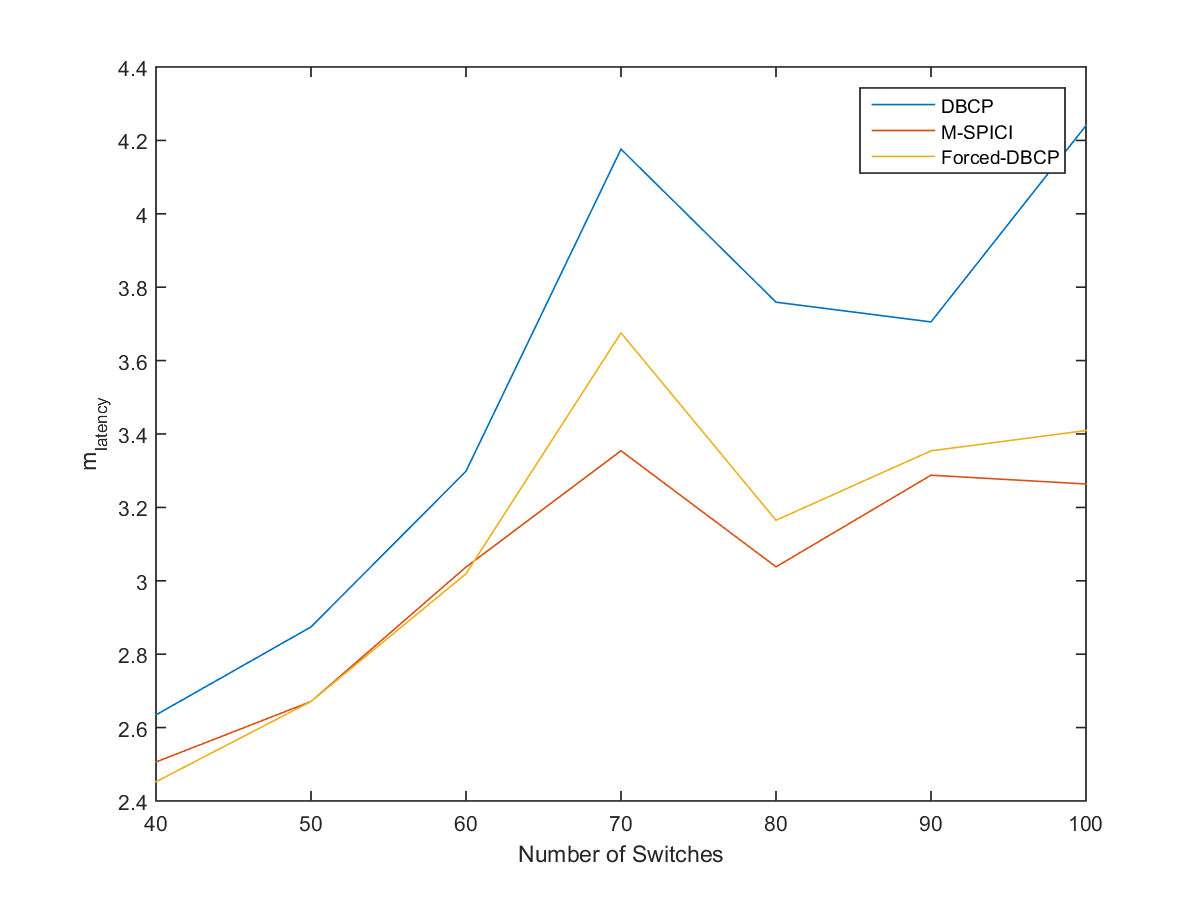
\includegraphics[width=\linewidth]{newgraph.png}
		\caption{Metric 1 vs No of switches}
		\label{fig:newgraph}
	\end{figure}

	In figure \ref{fig:newgraph} we used $m_{latency}$ or metric 1 as the comparison metric. We used Scenarios 1,2,3 and 5, which are all sparse graphs as our test cases. We evaluated the performance and compared 6 algorithms in the given figure.
	
	\begin{figure}
		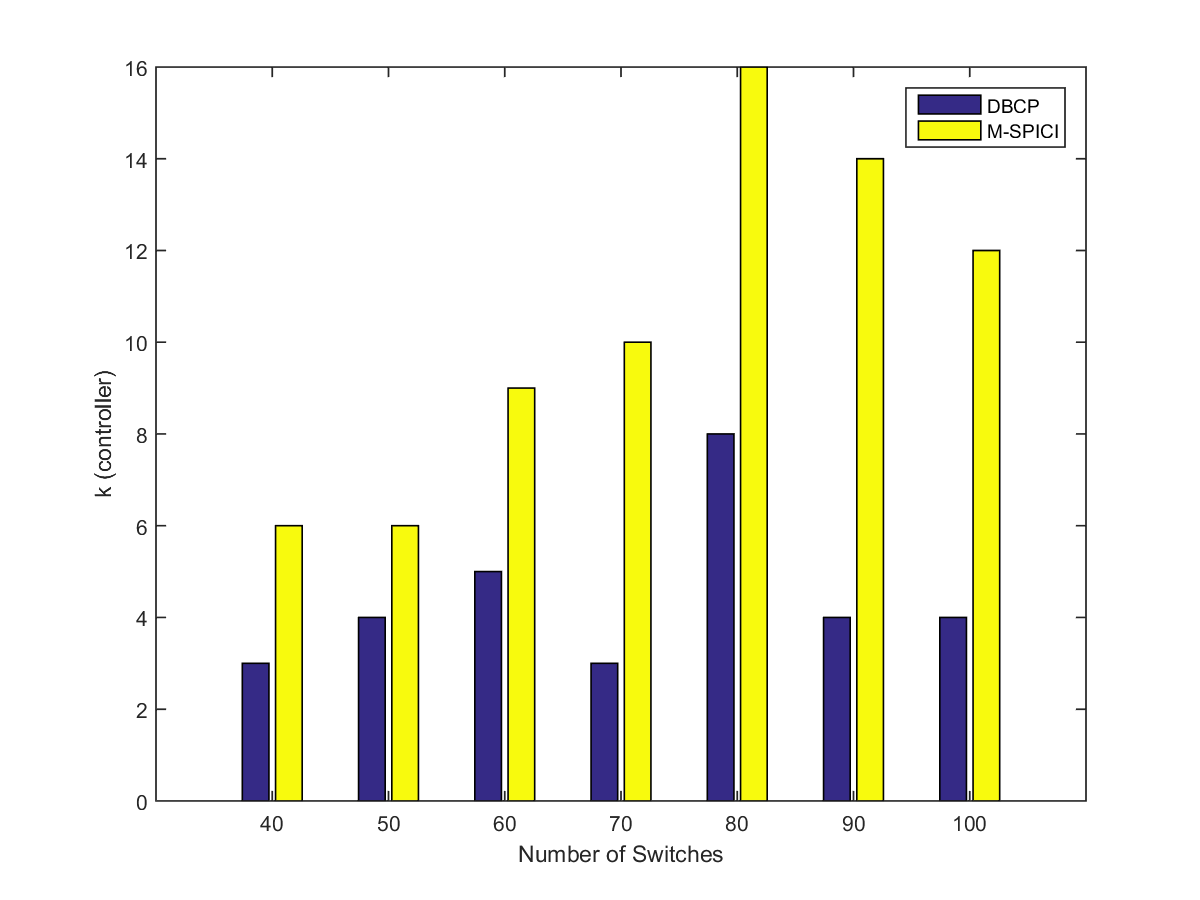
\includegraphics[width=\linewidth]{newbar.png}
		\caption{Metric 1 vs No of Edges \\ (1) Scenario 4  (2) Scenario 5  (3) Scenario 6  (4) Scenario 7}
		\label{fig:newbar}
	\end{figure}
	
	In figure \ref{fig:newbar} we used $m_{latency}$ again as the comparison metric. This time we used Scenarios 4,5,6 and 7, all of which contain 100 nodes and have different number of edges as our test cases. We evaluated the performance and compared 6 algorithms in the given figure.
	
	\begin{figure}
		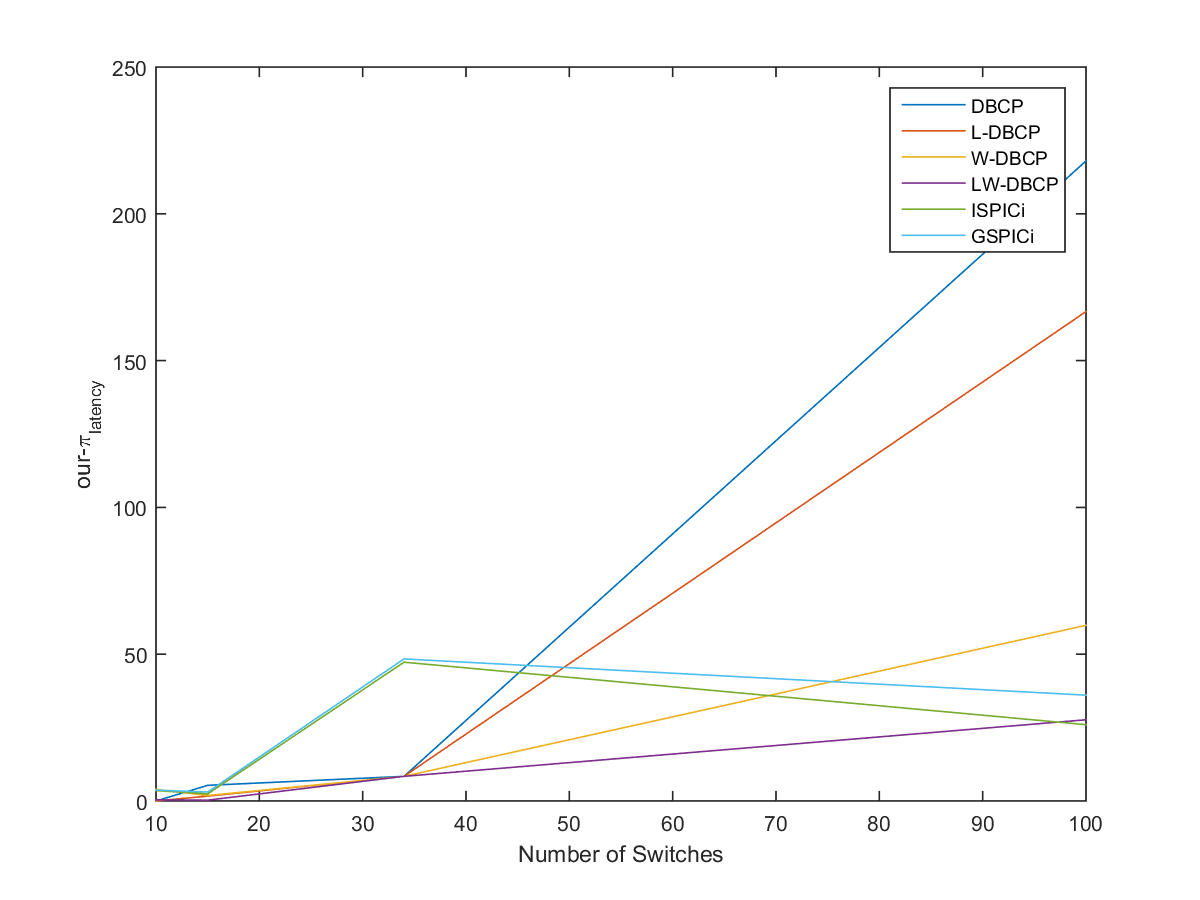
\includegraphics[width=\linewidth]{ourgraph.png}
		\caption{Metric 2 vs No of switches}
		\label{fig:ourgraph}
	\end{figure}
	
	In figure \ref{fig:ourgraph} we used $\pi_{latency}$ or metric 2 as the comparison metric. We used Scenarios 1,2,3 and 5, which are all sparse graphs as our test cases. We evaluated the performance and compared 6 algorithms in the given figure.
	
	\begin{figure}
		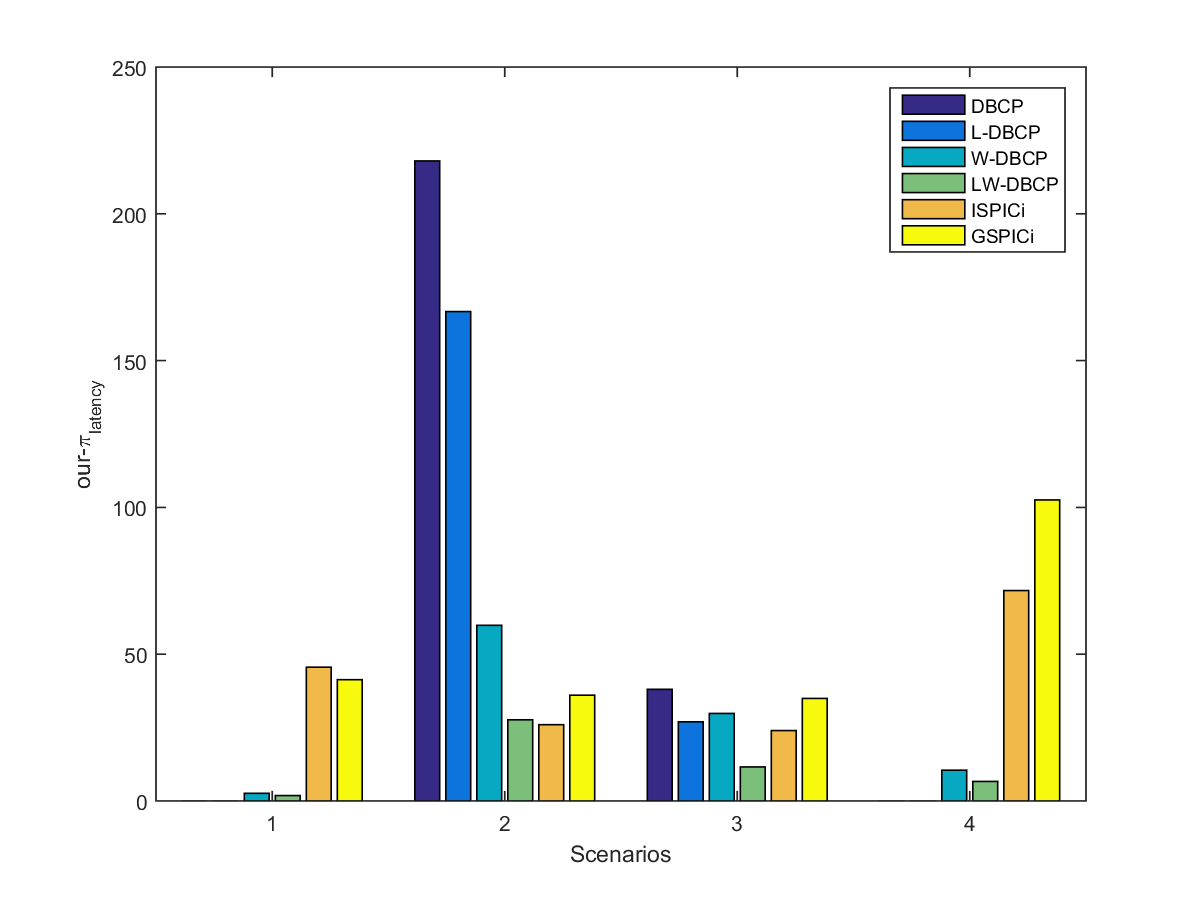
\includegraphics[width=\linewidth]{ourbar.png}
		\caption{Metric 2 vs No of Edges \\ (1) Scenario 4  (2) Scenario 5  (3) Scenario 6  (4) Scenario 7}
		\label{fig:ourbar}
	\end{figure}
	
	In figure \ref{fig:ourbar} we used $\pi_{latency}$ again as the comparison metric. This time we used Scenarios 4,5,6 and 7, all of which contain 100 nodes and have different number of edges as our test cases. We evaluated the performance and compared 6 algorithms in the given figure.
	
	\bibliographystyle{plain}
	\bibliography{references}
\end{document}